\section{ロジスティック回帰とパーセプトロン}
logistic regression, perceptron
1層パーセプトロン
\url{https://www.cs.utexas.edu/~gdurrett/courses/fa2022/perc-lr-connections.pdf}
\url{https://en.wikipedia.org/wiki/Perceptron}
\url{https://arxiv.org/abs/2012.03642}
perceptronは0/1 or -1/1のどちらか
UNDERSTANDING STRAIGHT-THROUGH ESTIMATOR IN TRAINING ACTIVATION QUANTIZED NEURAL NETS
Yoshua Bengio, Nicholas L´eonard, and Aaron Courville. Estimating or propagating gradients through stochastic neurons for conditional computation. arXiv preprint arXiv:1308.3432, 2013.
Hinton (2012) in his lecture 15b
G. Hinton. Neural networks for machine learning, 2012.
\url{https://www.cs.toronto.edu/~hinton/coursera_lectures.html}
delta rule
\begin{lstlisting}[language=julia]
using Random, PyPlot, ProgressMeter
rc("axes.spines", top=false, right=false)
\end{lstlisting}
\begin{lstlisting}[language=julia]
N = 400 # num of inputs
dims = 2  # dims of inputs 
Random.seed!(1234);
\end{lstlisting}
\begin{lstlisting}[language=julia]
X = [randn(Int(N/2), dims);  3.0 .+ randn(Int(N/2), dims)];
y = [zeros(Int(N/2)); ones(Int(N/2))];
\end{lstlisting}
\begin{lstlisting}[language=julia]
figure(figsize=(4, 4))
scatter(X[y.==0, 1], X[y.==0, 2])
scatter(X[y.==1, 1], X[y.==1, 2])
xlabel(L"$x_1$"); ylabel(L"$x_2$"); 
tight_layout()
\end{lstlisting}
\begin{figure}[ht]
	\centering
	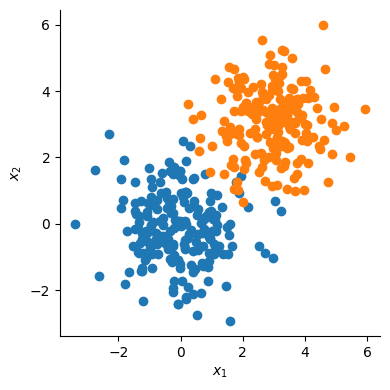
\includegraphics[scale=0.8, max width=\linewidth]{./fig/local-learning-rule/logistic-regression-perceptron/cell005.png}
	\caption{cell005.png}
	\label{cell005.png}
\end{figure}
\begin{lstlisting}[language=julia]
m, n = 2, 1
\end{lstlisting}
\begin{lstlisting}[language=julia]
step(x) = 1.0(x > 0)
\end{lstlisting}
\begin{lstlisting}[language=julia]
x = -1:0.01:1
figure(figsize=(3, 2))
plot(x, step.(x))
tight_layout()
\end{lstlisting}
\begin{figure}[ht]
	\centering
	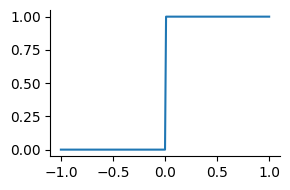
\includegraphics[scale=0.8, max width=\linewidth]{./fig/local-learning-rule/logistic-regression-perceptron/cell008.png}
	\caption{cell008.png}
	\label{cell008.png}
\end{figure}
Here σ denotes the (point-wise) activation function, $W \in R^{m\times n}$
is the weight-matrix and $b \in R^n$
is
the bias-vector. The vector $x \in R^m$ and the vector $y \in R^n$ denote the input, respectively the output
\begin{equation}
y=\sigma(W^\top x + b)
\end{equation}
\begin{align}
& \text { Initialize } W^0, b^0 \text {; } \\
& \text { for } k=1,2, \ldots \text { do } \\
& \qquad \begin{array}{|l}
\text { for } i=1, \ldots, s \text { do } \\
e_i=y_i-\sigma\left(\left(W^k\right)^{\top} x_i+b^k\right) \\
W^{k+1}=W^k+e_i x_i^{\top} \\
b^{k+1}=b^k+e_i
\end{array} \\
& \text { end }
\end{align}
\begin{lstlisting}[language=julia]
n_iter = 100
loss = zeros(n_iter);
W = randn(n, m)
b = randn(n)
for t in 1:n_iter
    ŷ = step.(W * X' .+ b)'
    e = y - ŷ
    loss[t] = sum(e.^2) 
    W[:, :] += 0.1*(1/200) * e' * X
    b[:] .+= 0.1*(1/200) * sum(e)
end
\end{lstlisting}
\begin{lstlisting}[language=julia]
figure(figsize=(3,2))
plot(loss)
xlabel("Iteration"); ylabel("Loss")
tight_layout()
\end{lstlisting}
\begin{figure}[ht]
	\centering
	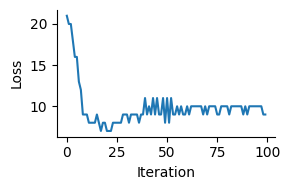
\includegraphics[scale=0.8, max width=\linewidth]{./fig/local-learning-rule/logistic-regression-perceptron/cell011.png}
	\caption{cell011.png}
	\label{cell011.png}
\end{figure}
\begin{lstlisting}[language=julia]
ŷ = step.(W * X' .+ b)'; # prediction
\end{lstlisting}
\begin{lstlisting}[language=julia]
p1 = X[ŷ[:, 1] .== 0, :]
p2 = X[ŷ[:, 1] .== 1, :];
\end{lstlisting}
ax + by + c = 0  
y = -a/b x - c/b
\begin{lstlisting}[language=julia]
xx = -3:0.01:6
yy = -W[1]/W[2]*xx .- b / W[2];
\end{lstlisting}
\begin{lstlisting}[language=julia]
figure(figsize=(4, 4))
scatter(p1[:, 1], p1[:, 2])
scatter(p2[:, 1], p2[:, 2])
plot(xx, yy, color="k")
xlabel(L"$x_1$"); ylabel(L"$x_2$"); 
tight_layout()
\end{lstlisting}
\begin{figure}[ht]
	\centering
	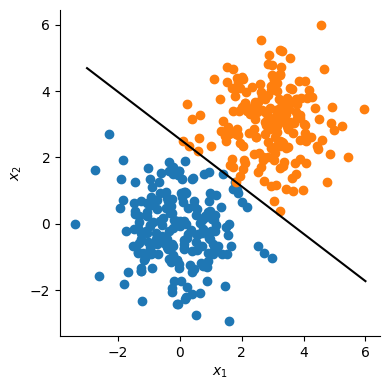
\includegraphics[scale=0.8, max width=\linewidth]{./fig/local-learning-rule/logistic-regression-perceptron/cell016.png}
	\caption{cell016.png}
	\label{cell016.png}
\end{figure}
